\chapter{Findings After User Testing}

To validate the usefulness and usability of Jadwal, we conducted a survey among friends, family, and early testers after they used the app. The results were highly positive and confirmed many of our original assumptions. This section presents a summary of the insights gained from the survey responses.

\begin{figure}[H]
\centering
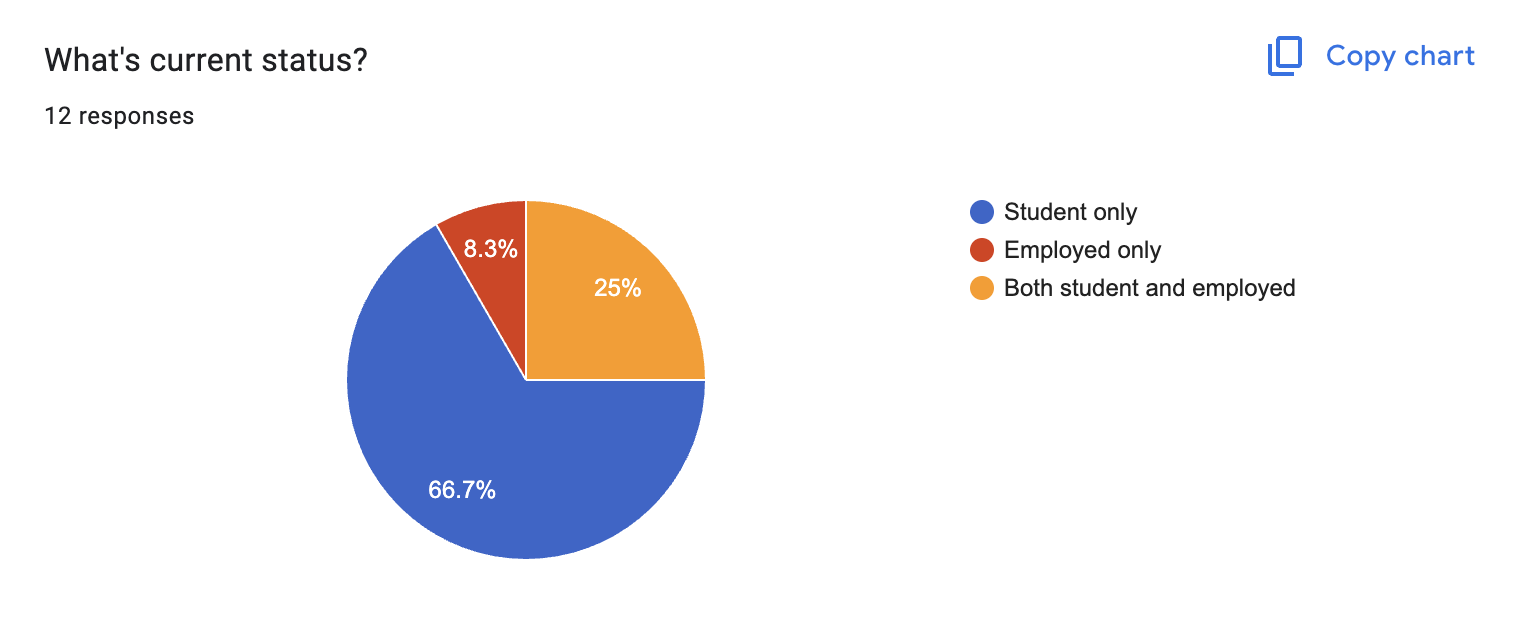
\includegraphics[width=0.8\textwidth]{images/end-survey/01-current-status.png}
\caption{Current Status of Respondents}
\label{fig:current-status}
\end{figure}

Figure~\ref{fig:current-status} shows that 66.7\% of respondents were students, 25\% were both students and employed, and 8.3\% were employed only.

\begin{figure}[H]
\centering
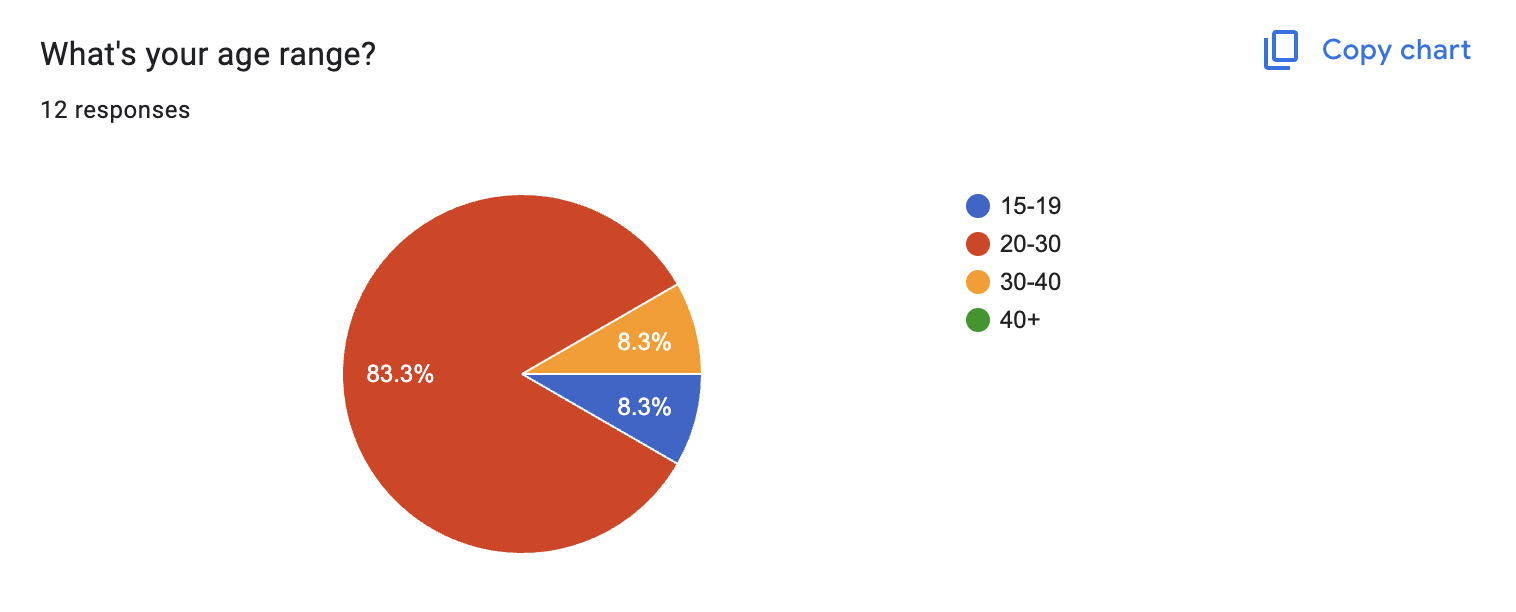
\includegraphics[width=0.8\textwidth]{images/end-survey/02-age-range.png}
\caption{Age Distribution}
\label{fig:age-range}
\end{figure}

As shown in Figure~\ref{fig:age-range}, the majority of participants (83.3\%) fell within the 20–30 age group, which aligns with our target demographic.

\begin{figure}[H]
\centering
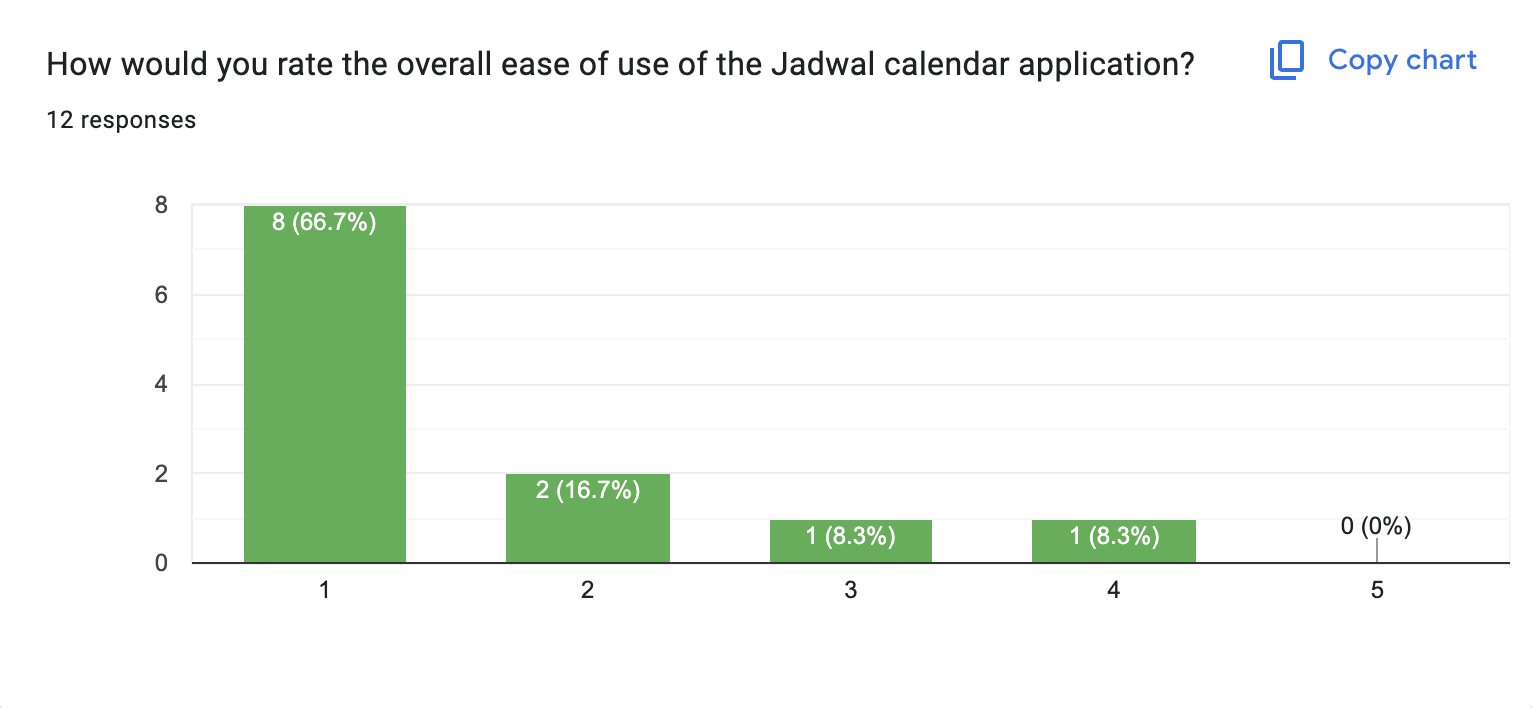
\includegraphics[width=0.8\textwidth]{images/end-survey/03-ease-of-use.png}
\caption{Ease of Use}
\label{fig:ease-of-use}
\end{figure}

According to Figure~\ref{fig:ease-of-use}, 66.7\% rated the app as extremely easy to use (1 on a 5-point scale).

\begin{figure}[H]
\centering
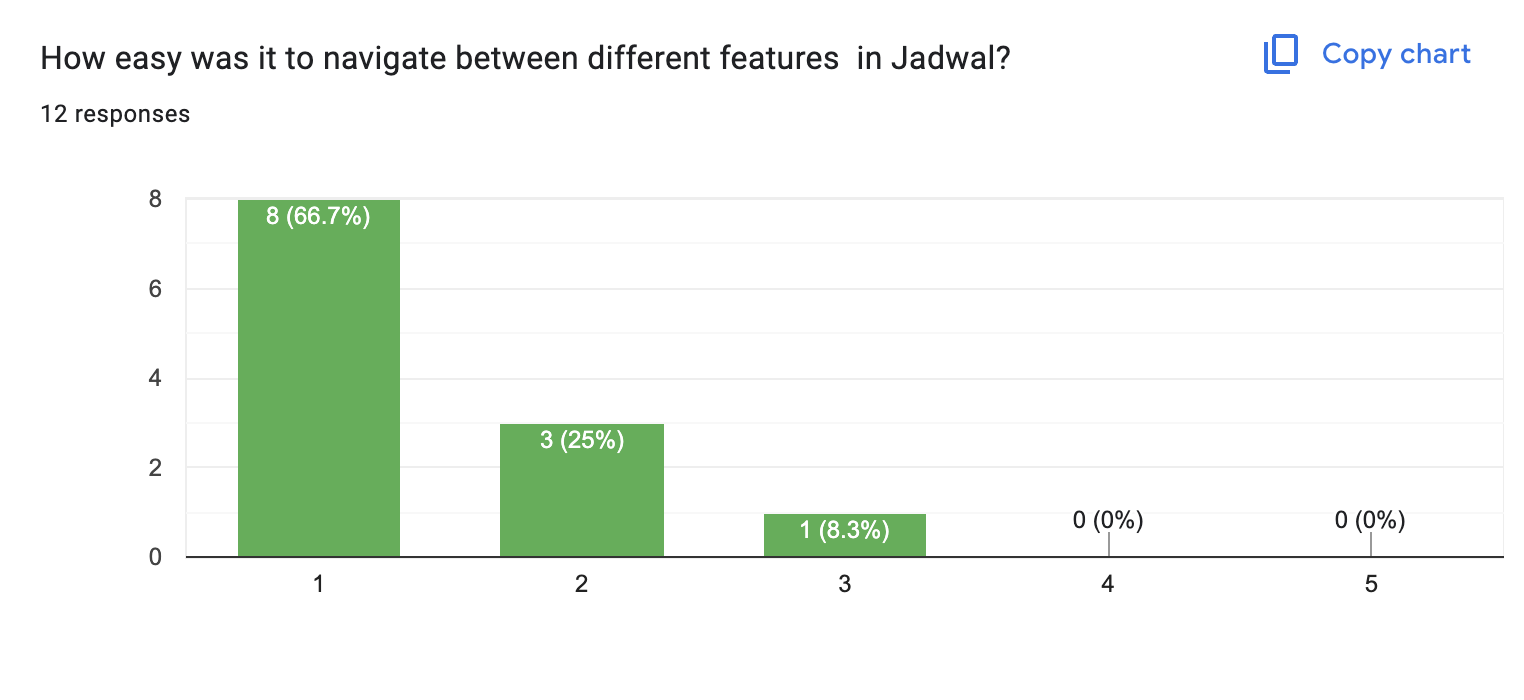
\includegraphics[width=0.8\textwidth]{images/end-survey/04-ease-of-feature-navigation.png}
\caption{Ease of Navigating Features}
\label{fig:ease-of-feature-navigation}
\end{figure}

As seen in Figure~\ref{fig:ease-of-feature-navigation}, 66.7\% of users reported that navigating between features was very intuitive.

\begin{figure}[H]
\centering
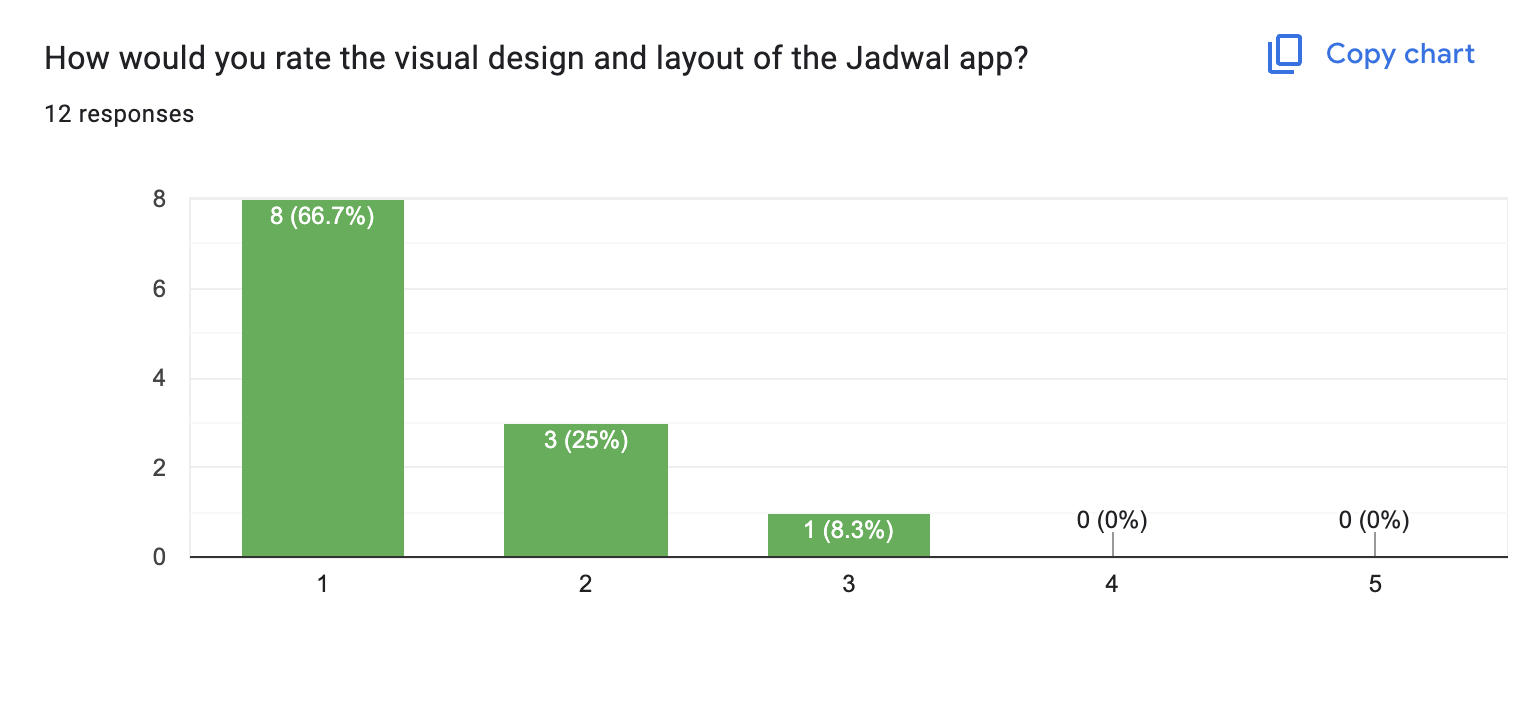
\includegraphics[width=0.8\textwidth]{images/end-survey/05-visual-design-rate.png}
\caption{Visual Design Satisfaction}
\label{fig:visual-design-rate}
\end{figure}

Figure~\ref{fig:visual-design-rate} indicates that 66.7\% of participants rated the app’s design and layout as excellent.

\begin{figure}[H]
\centering
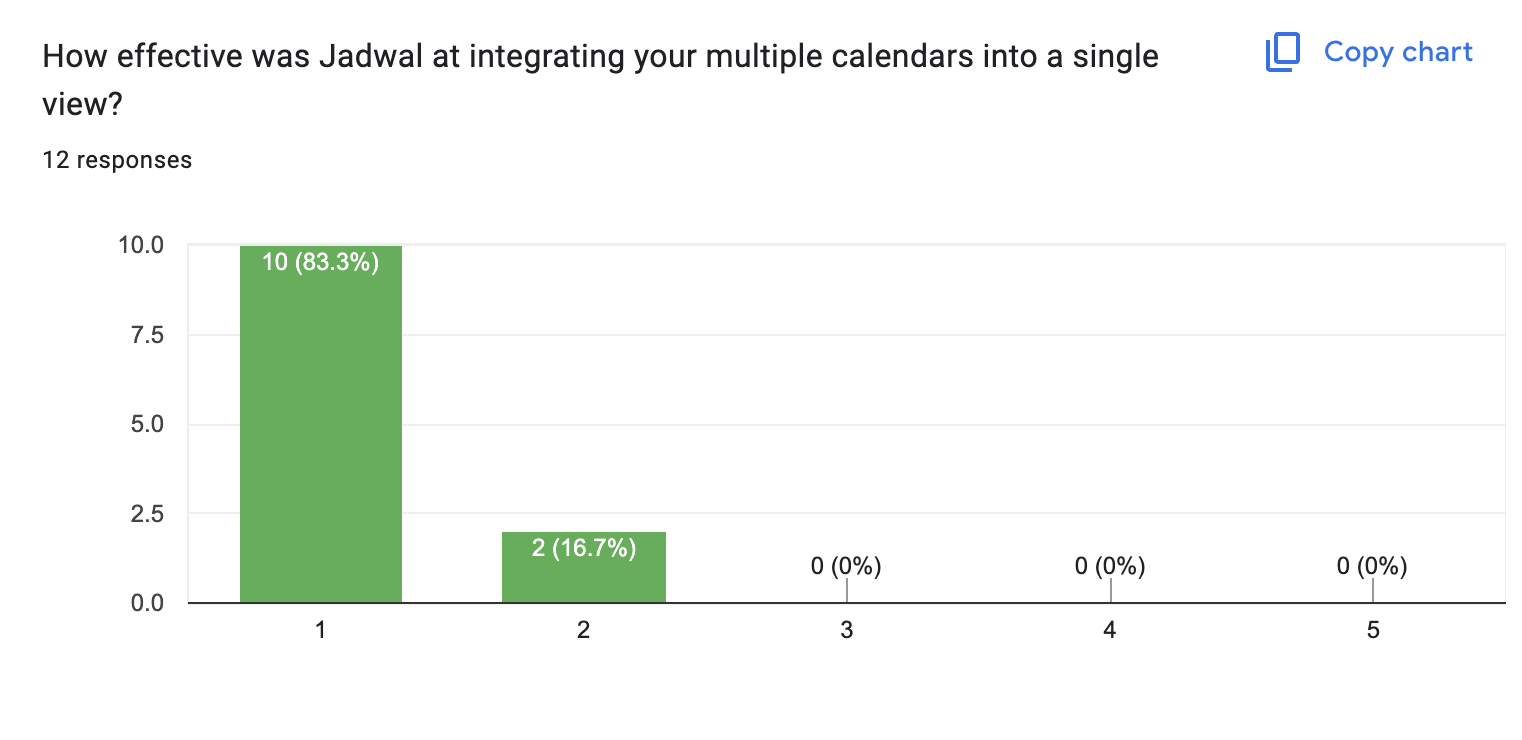
\includegraphics[width=0.8\textwidth]{images/end-survey/06-jadwal-effectiveness-integrating-multiple-calendars.png}
\caption{Effectiveness in Integrating Calendars}
\label{fig:jadwal-effectiveness-integrating-multiple-calendars}
\end{figure}

Figure~\ref{fig:jadwal-effectiveness-integrating-multiple-calendars} shows that 83.3\% found Jadwal effective at integrating multiple calendars into one interface.

\begin{figure}[H]
\centering
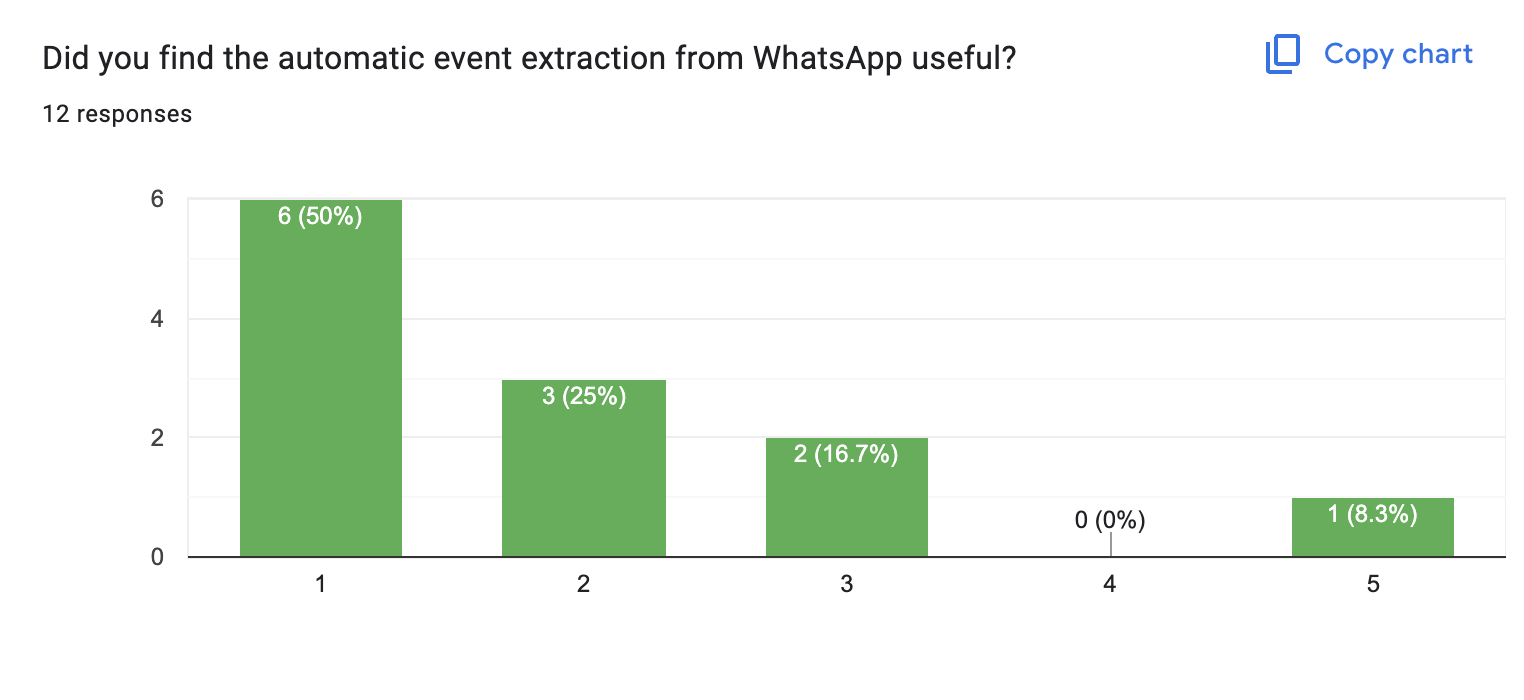
\includegraphics[width=0.8\textwidth]{images/end-survey/07-automatic-event-extraction.png}
\caption{Usefulness of Automatic Event Extraction}
\label{fig:automatic-event-extraction}
\end{figure}

Half of the users (50\%) found WhatsApp-based automatic event extraction very useful (Figure~\ref{fig:automatic-event-extraction}), while 25\% rated it slightly less positively, and 8.3\% reported it was not useful.

\begin{figure}[H]
\centering
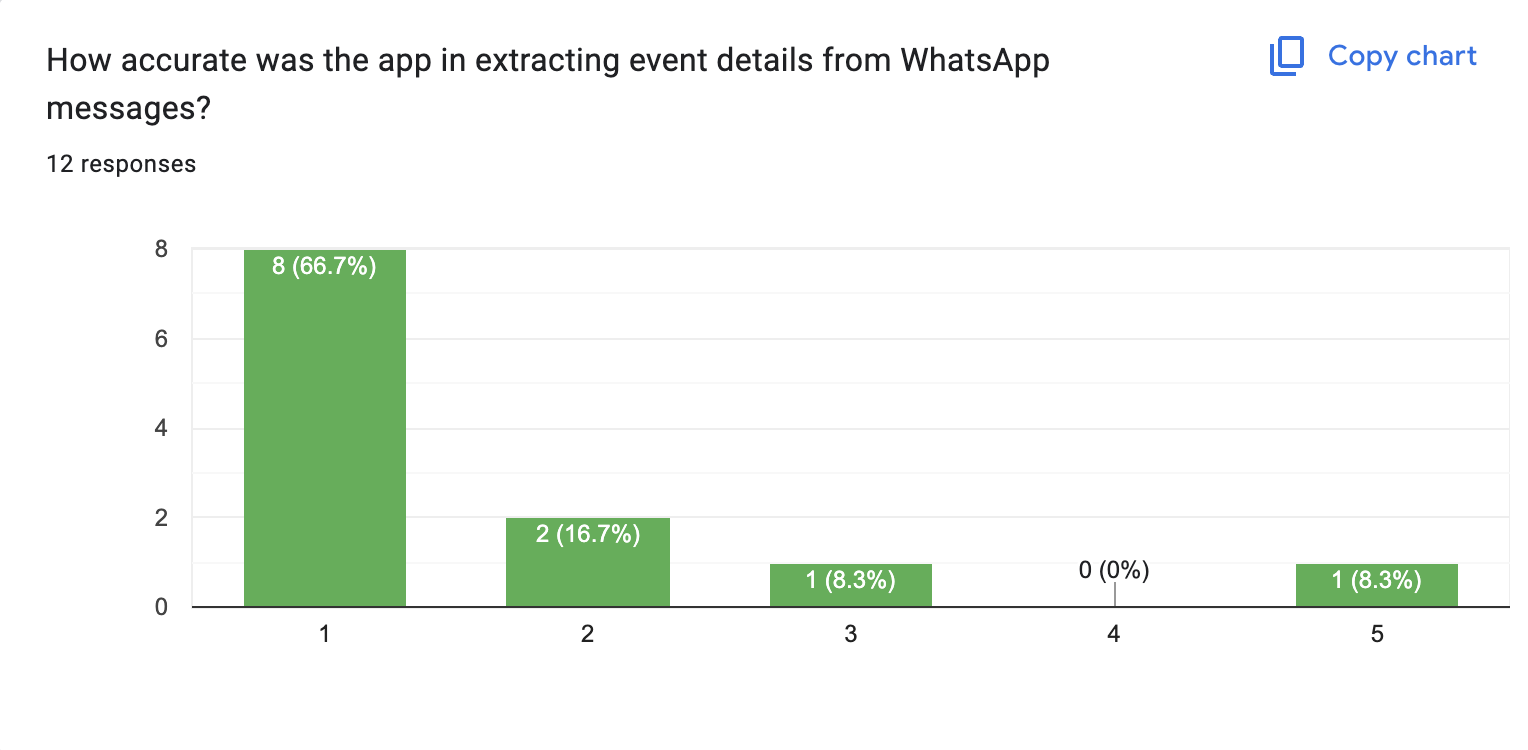
\includegraphics[width=0.8\textwidth]{images/end-survey/08-accuracy-of-extraction.png}
\caption{Accuracy of Extracted Events}
\label{fig:accuracy-of-extraction}
\end{figure}

In Figure~\ref{fig:accuracy-of-extraction}, 66.7\% confirmed that extracted events were accurate, while a small minority gave low scores.

\begin{figure}[H]
\centering
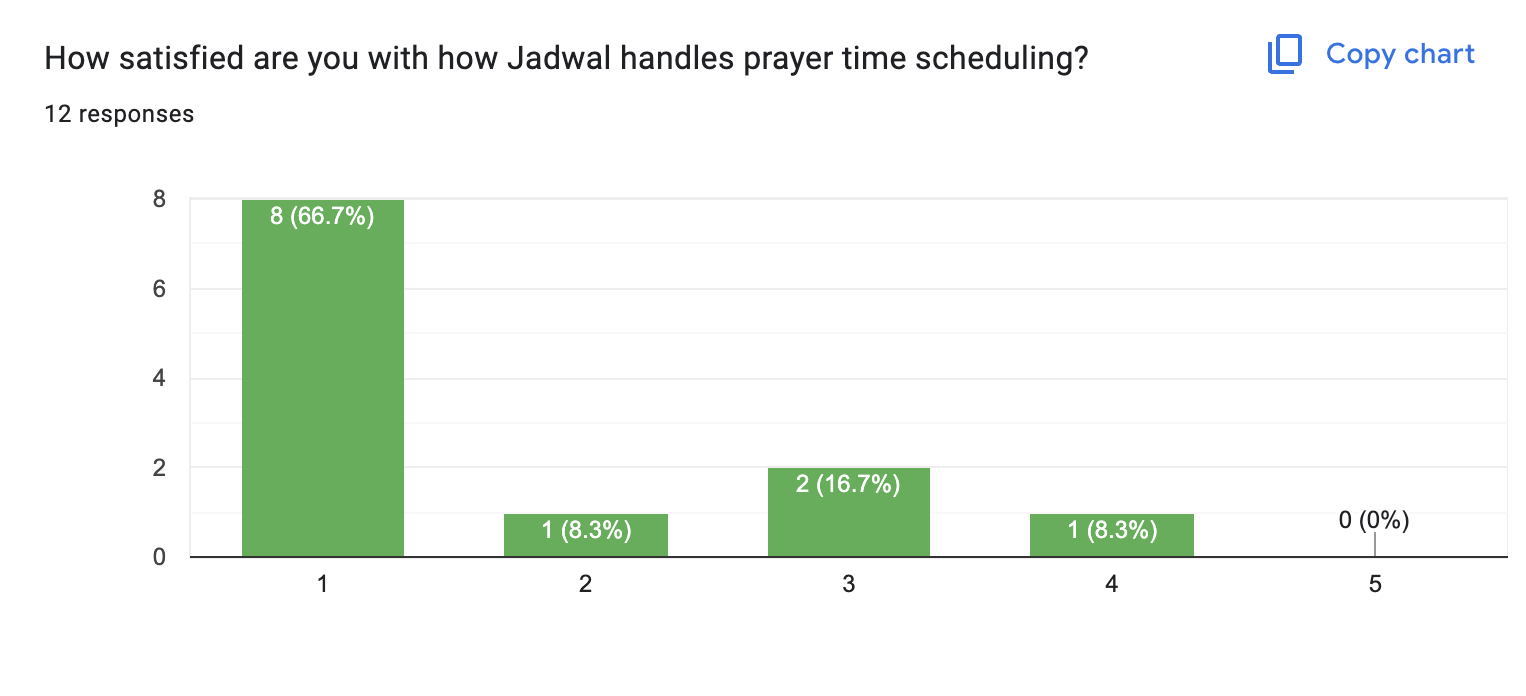
\includegraphics[width=0.8\textwidth]{images/end-survey/09-satisfaction-with-prayer-times.png}
\caption{Satisfaction with Prayer Time Scheduling}
\label{fig:satisfaction-with-prayer-times}
\end{figure}

Figure~\ref{fig:satisfaction-with-prayer-times} shows that 66.7\% were highly satisfied with the prayer time scheduling feature, and 16.7\% were neutral.

\begin{figure}[H]
\centering
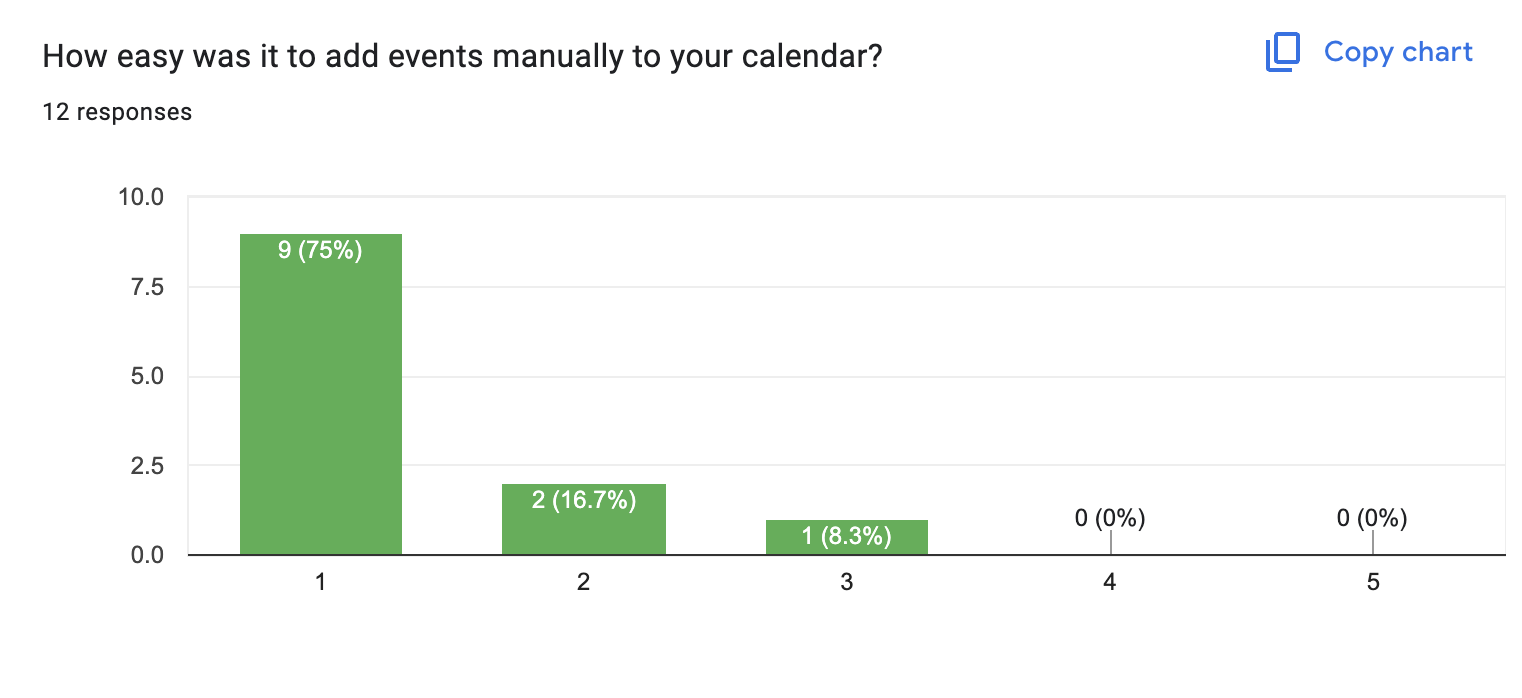
\includegraphics[width=0.8\textwidth]{images/end-survey/10-ease-of-adding-events-manually.png}
\caption{Ease of Manually Adding Events}
\label{fig:ease-of-adding-events-manually}
\end{figure}

As shown in Figure~\ref{fig:ease-of-adding-events-manually}, 75\% found manual event creation straightforward and easy.

\begin{figure}[H]
\centering
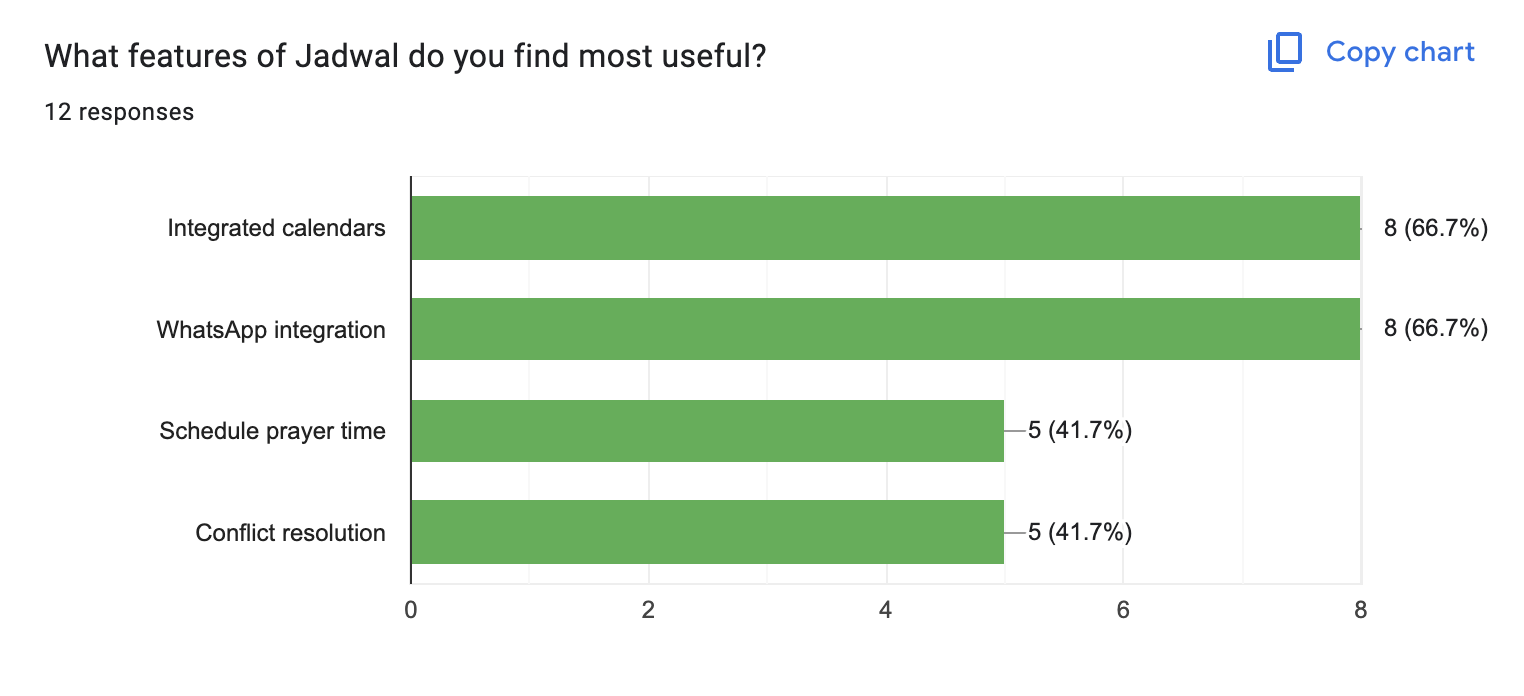
\includegraphics[width=0.8\textwidth]{images/end-survey/11-most-useful-feature.png}
\caption{Most Useful Features}
\label{fig:most-useful-feature}
\end{figure}

Figure~\ref{fig:most-useful-feature} reveals that calendar integration and WhatsApp event extraction were considered the most useful features by 66.7\% of users, while prayer time scheduling and conflict resolution were each mentioned by 41.7\%.

\begin{figure}[H]
\centering
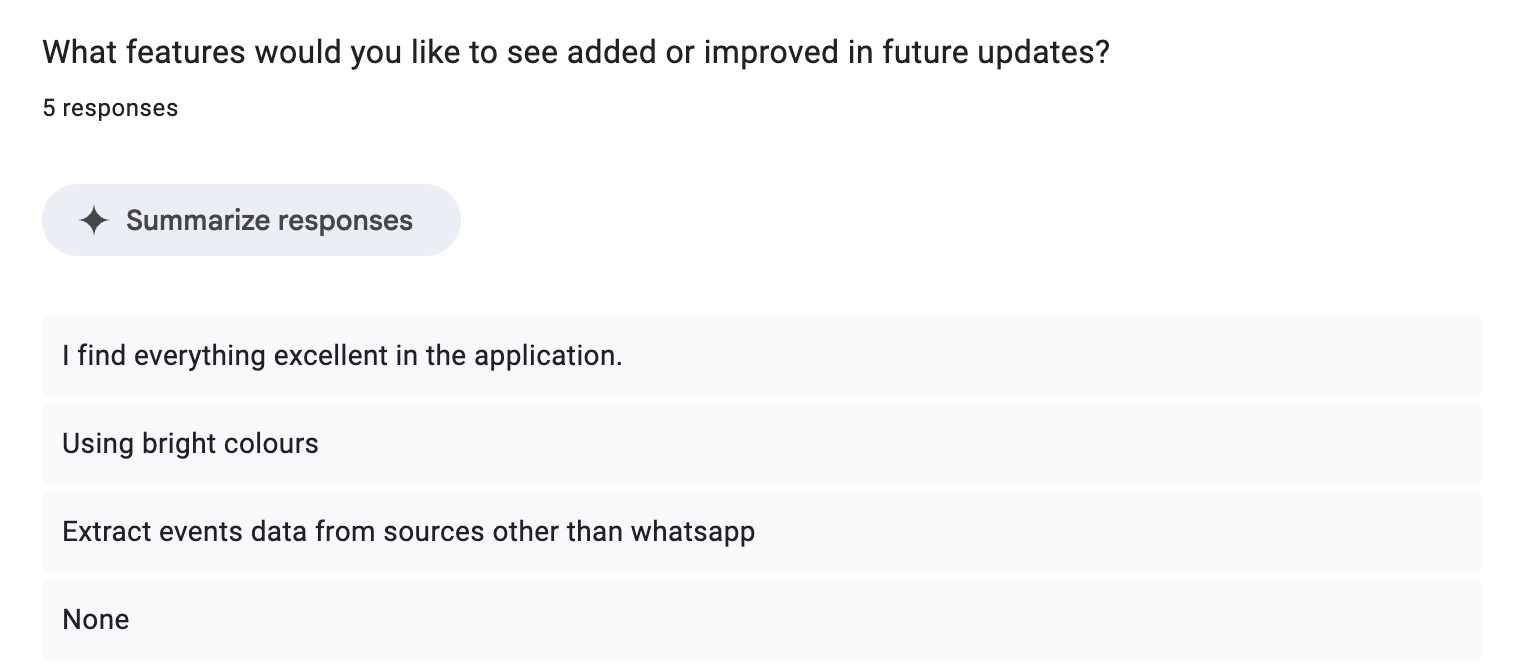
\includegraphics[width=0.8\textwidth]{images/end-survey/12-features-you-like-be-added.png}
\caption{Requested Features}
\label{fig:features-you-like-be-added}
\end{figure}

Respondents suggested features such as support for more messaging apps, UI enhancements (e.g., brighter colors), and improvements to event detection (Figure~\ref{fig:features-you-like-be-added}).

\begin{figure}[H]
\centering
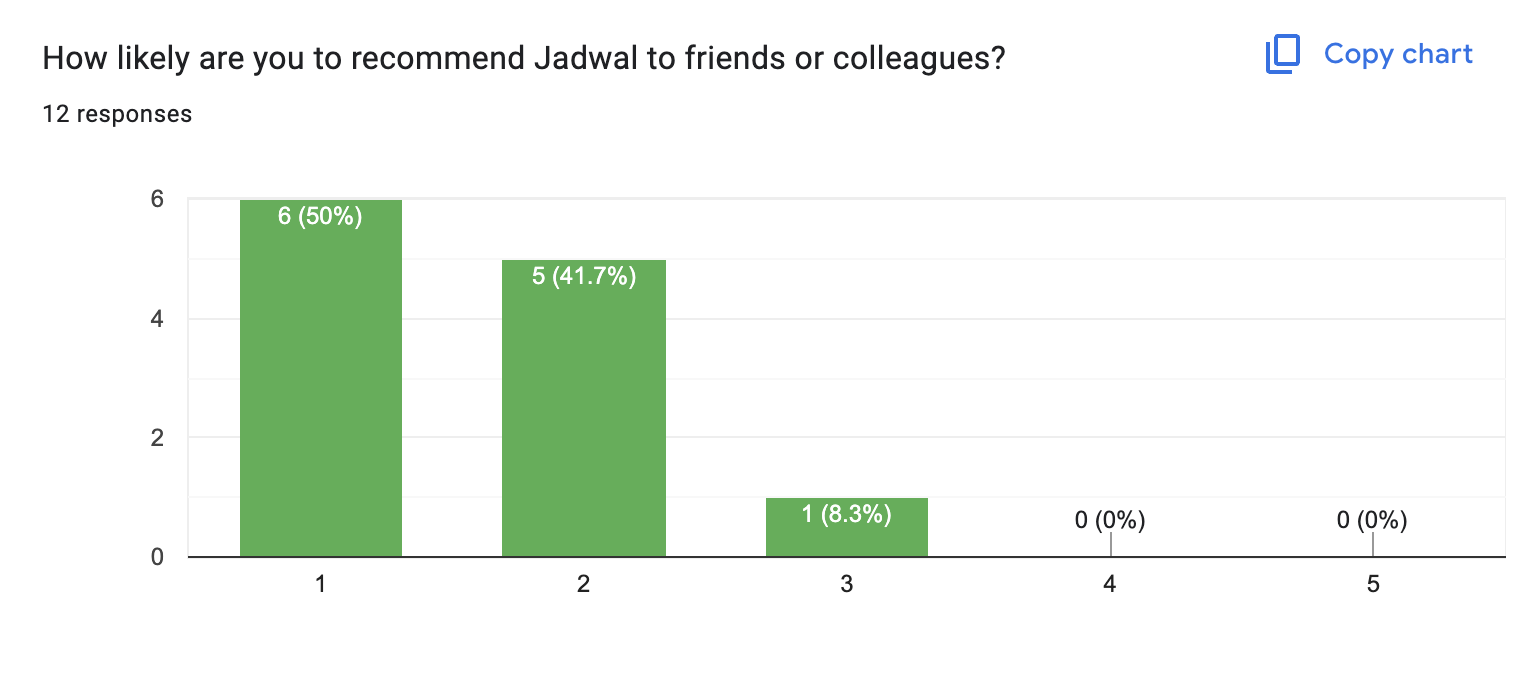
\includegraphics[width=0.8\textwidth]{images/end-survey/13-likely-to-recommend.png}
\caption{Likelihood to Recommend Jadwal}
\label{fig:likely-to-recommend}
\end{figure}

According to Figure~\ref{fig:likely-to-recommend}, half of the respondents (50\%) were extremely likely to recommend Jadwal to others.

\begin{figure}[H]
\centering
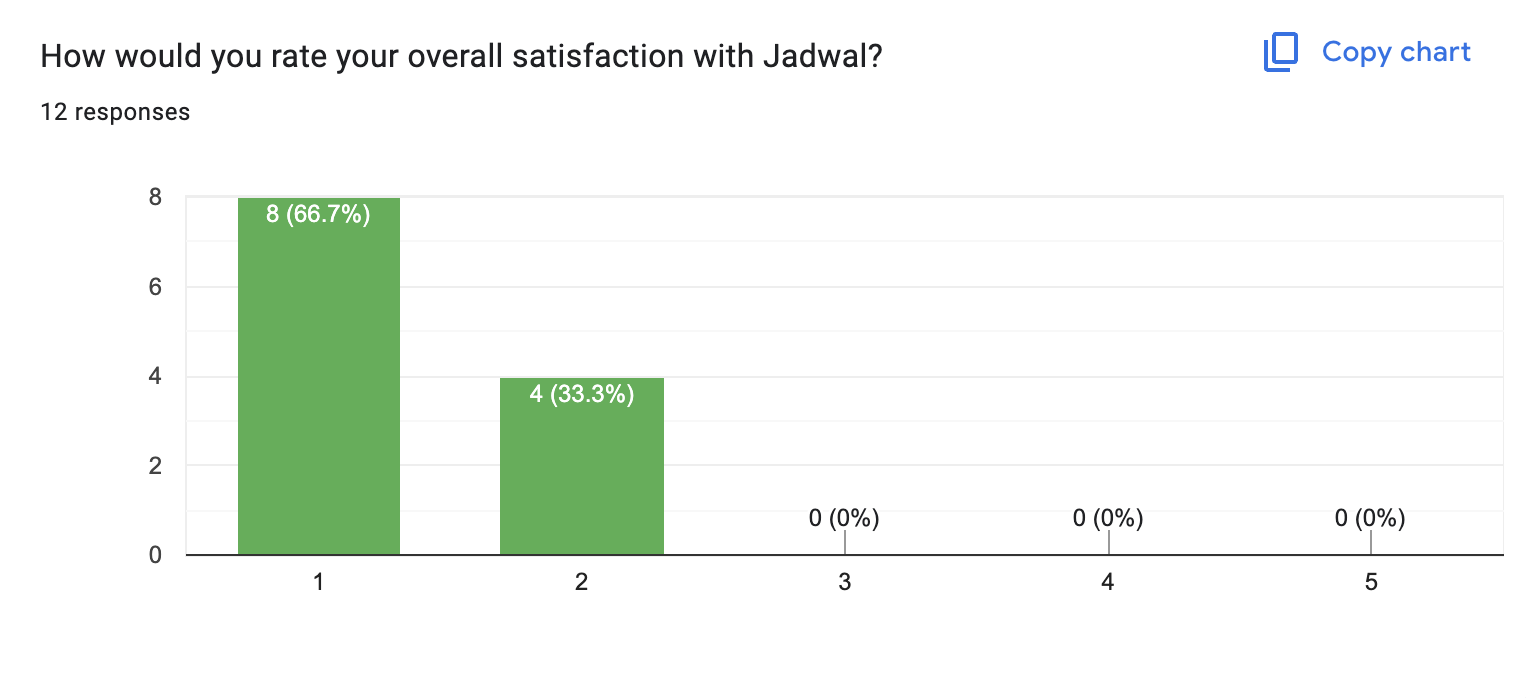
\includegraphics[width=0.8\textwidth]{images/end-survey/14-overall-satsifacation.png}
\caption{Overall Satisfaction}
\label{fig:overall-satsifacation}
\end{figure}

Finally, as shown in Figure~\ref{fig:overall-satsifacation}, 66.7\% of users expressed extremely high overall satisfaction with the app.